% !TeX root = ../main.tex
% Add the above to each chapter to make compiling the PDF easier in some editors.

\chapter{Performance testing setup} \label{benchmark_setup}
As can be gathered from the previous chapters, the optimizations implemented in Tachyon for this thesis are 
\begin{itemize}
\item Superfrustum Culling
\item (vendor agnostic) Multiview Stereo Rendering
\item \gls{HMD}-matched Stencil Mask
\item Monoscopic Far-Field Rendering
\end{itemize}

While expectations for the first three items were optimistic, it shall be noted again that MFFR unfortunately turned out unsuccessful, which will reflect in this following chapter. 

\section{Benchmark scene}
In order to properly assess how each of these implementations fares at run-time and how it impacts performance of the engine, a series of benchmarks were conducted. To ensure repeatability of the benchmark, a synthetic test scene was constructed, aimed to stress the tested systems to a degree not likely found in many real scenarios. While this may seem counterintuitive, it paints a worst-case picture of performance to be expected and how the tested methods hold up. \\
This test scene is built as follows: the scene dimensions are set up as 32 by 32 \codeword{chunk}s, each \codeword{chunk} sized 80 units on each axis. This gives an overall scene volume of 2560 by 80 by 2560 units. This seems strongly skewed towards lateral expansion rather than vertical, chosen primarily due to the expected productive use being industrial scenes covering large factory floors but not necessarily very vertical setups. Another reason is that the Tachyon scene \codeword{chunk} system currently does not allow stacking of \codeword{chunk}s and as such an adequate compromise between scene scale and octree scale had to be chosen. 
Filling this test scene is a selection of objects, the geometries namely being a primitive cube and three high polycount objects, a robot called "Robi", a material showcase sphere and a PBR showcase helmet. While such condensed high detail polygon amounts are not an ideal showcase, they provide enough geometry load (large number of triangles, \autoref{fig:highpolys}) for a synthetic test. As culling is done not per object but per octree cell, the distribution of geometry within small spaces is a lesser issue and the overall distribution achieved here is consistent enough for tangible testing. These objects are placed in the scene by iterating through a counter for each axis and placing an object instance at each new count. To determine the instance position, the three axis counts at that moment are multiplied by a spacing of 3.6 and a entropy value is added to each axis. This entropy value is combined as \codeword{x = sinf(sinf(x) + cosf(y) + tanf(z))}, \codeword{y = cosf(sinf(y) + cosf(z) + tanf(x))}, \codeword{z = sinf(cosf(sinf(z) + cosf(x) + tanf(y)))}. Adding this artificial entropy makes the scene look more chaotic but is still deterministic and repeatable.
By default the placed object is a primitive cube, but at every intersection of x+z, y-z and z counts valued 11, one high polycount instance is placed, with the chosen type being modulo-index-incremented over the available high polycount types. 
This placement setup is done with target counts of 711 for the X and Z and 22 for the Y axis respectively. This utilizes the scene height as much as possible and results in a total instance count of 11.121.462, a respectable number even for detailed industrial applications. In a flythrough in the 2D mirror viewport, the scene looks as shown in \autoref{fig:scene_chaos_2}. \\
Still in the interest of repeatability, the head-tracked headset pose is disabled for these tests in favor of a scripted on-rails camera pose that follows a simple circular pattern for its virtual position and another one for rotation, both based on the sine and cosine of the number of frames completed since the first rendered frame. This gives a simple and arbitrarily repeatable pattern resulting in the same camera position and angle at the same frame count for each run, obviously making it much easier to match measurements. 

\iffalse
\begin{figure}[htb]
  \centering
  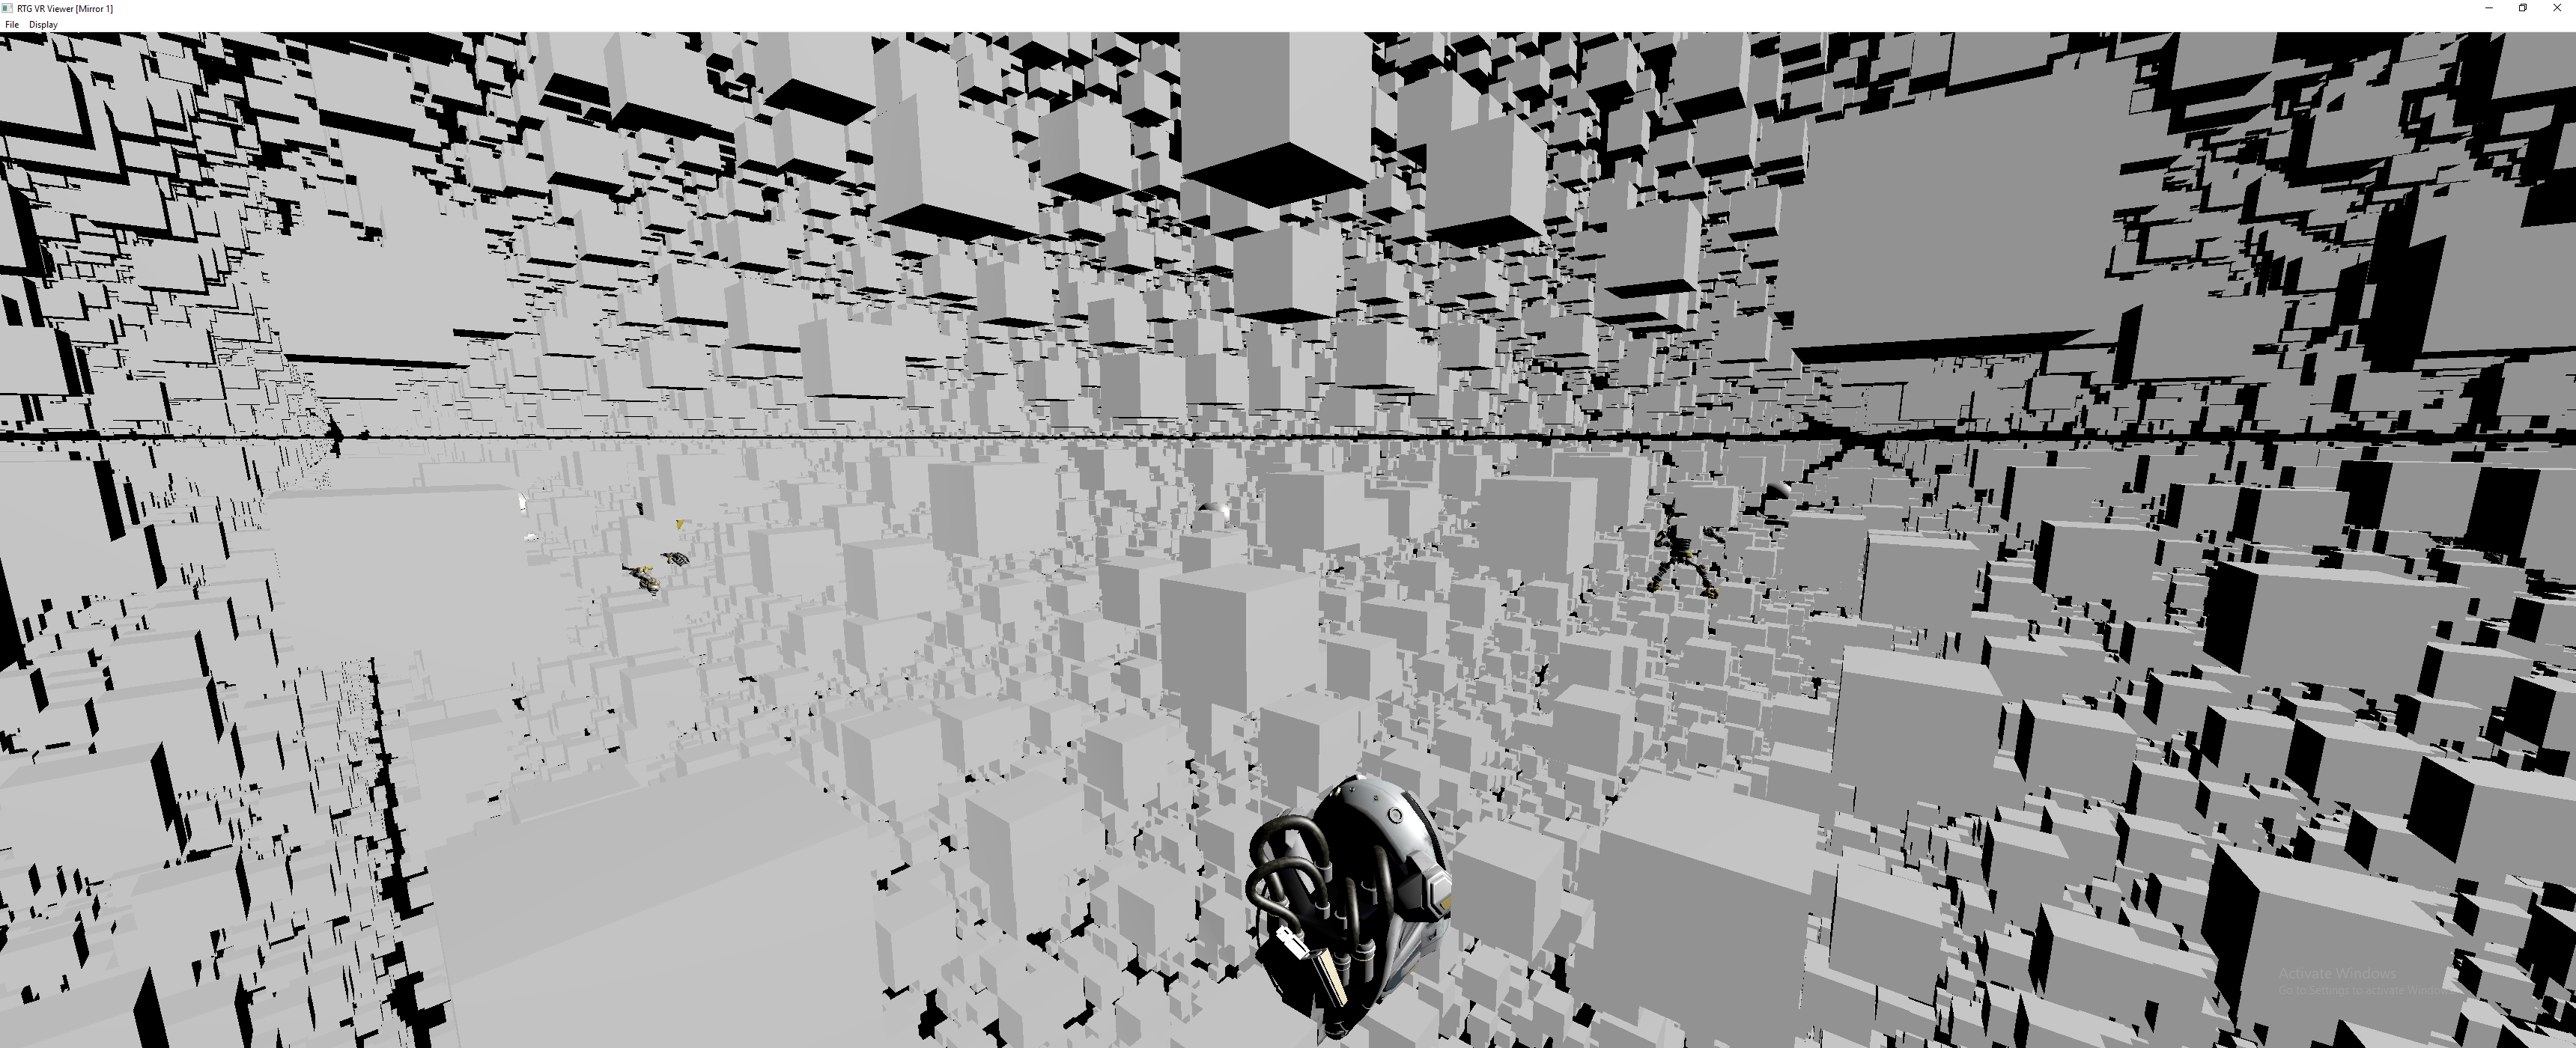
\includegraphics[width=0.9\textwidth]{pictures/scene_chaos}
  \caption{Sample scene with high object density, far draw distance and high degree of overdraw when rendered without per-frame Z ordering, screenshot taken of \gls{Tachyon}'s desktop viewport (repetition of \autoref{fig:scene_chaos})} \label{fig:scene_chaos_2}
\end{figure}
\fi

\begin{figure}[!ht]
  \centering
     \subfloat[Sample scene with high object density, far draw distance and high degree of overdraw when rendered without per-frame Z ordering, screenshot taken of \gls{Tachyon}'s desktop viewport (repetition of \autoref{fig:scene_chaos})\label{fig:scene_chaos_2}]{%
       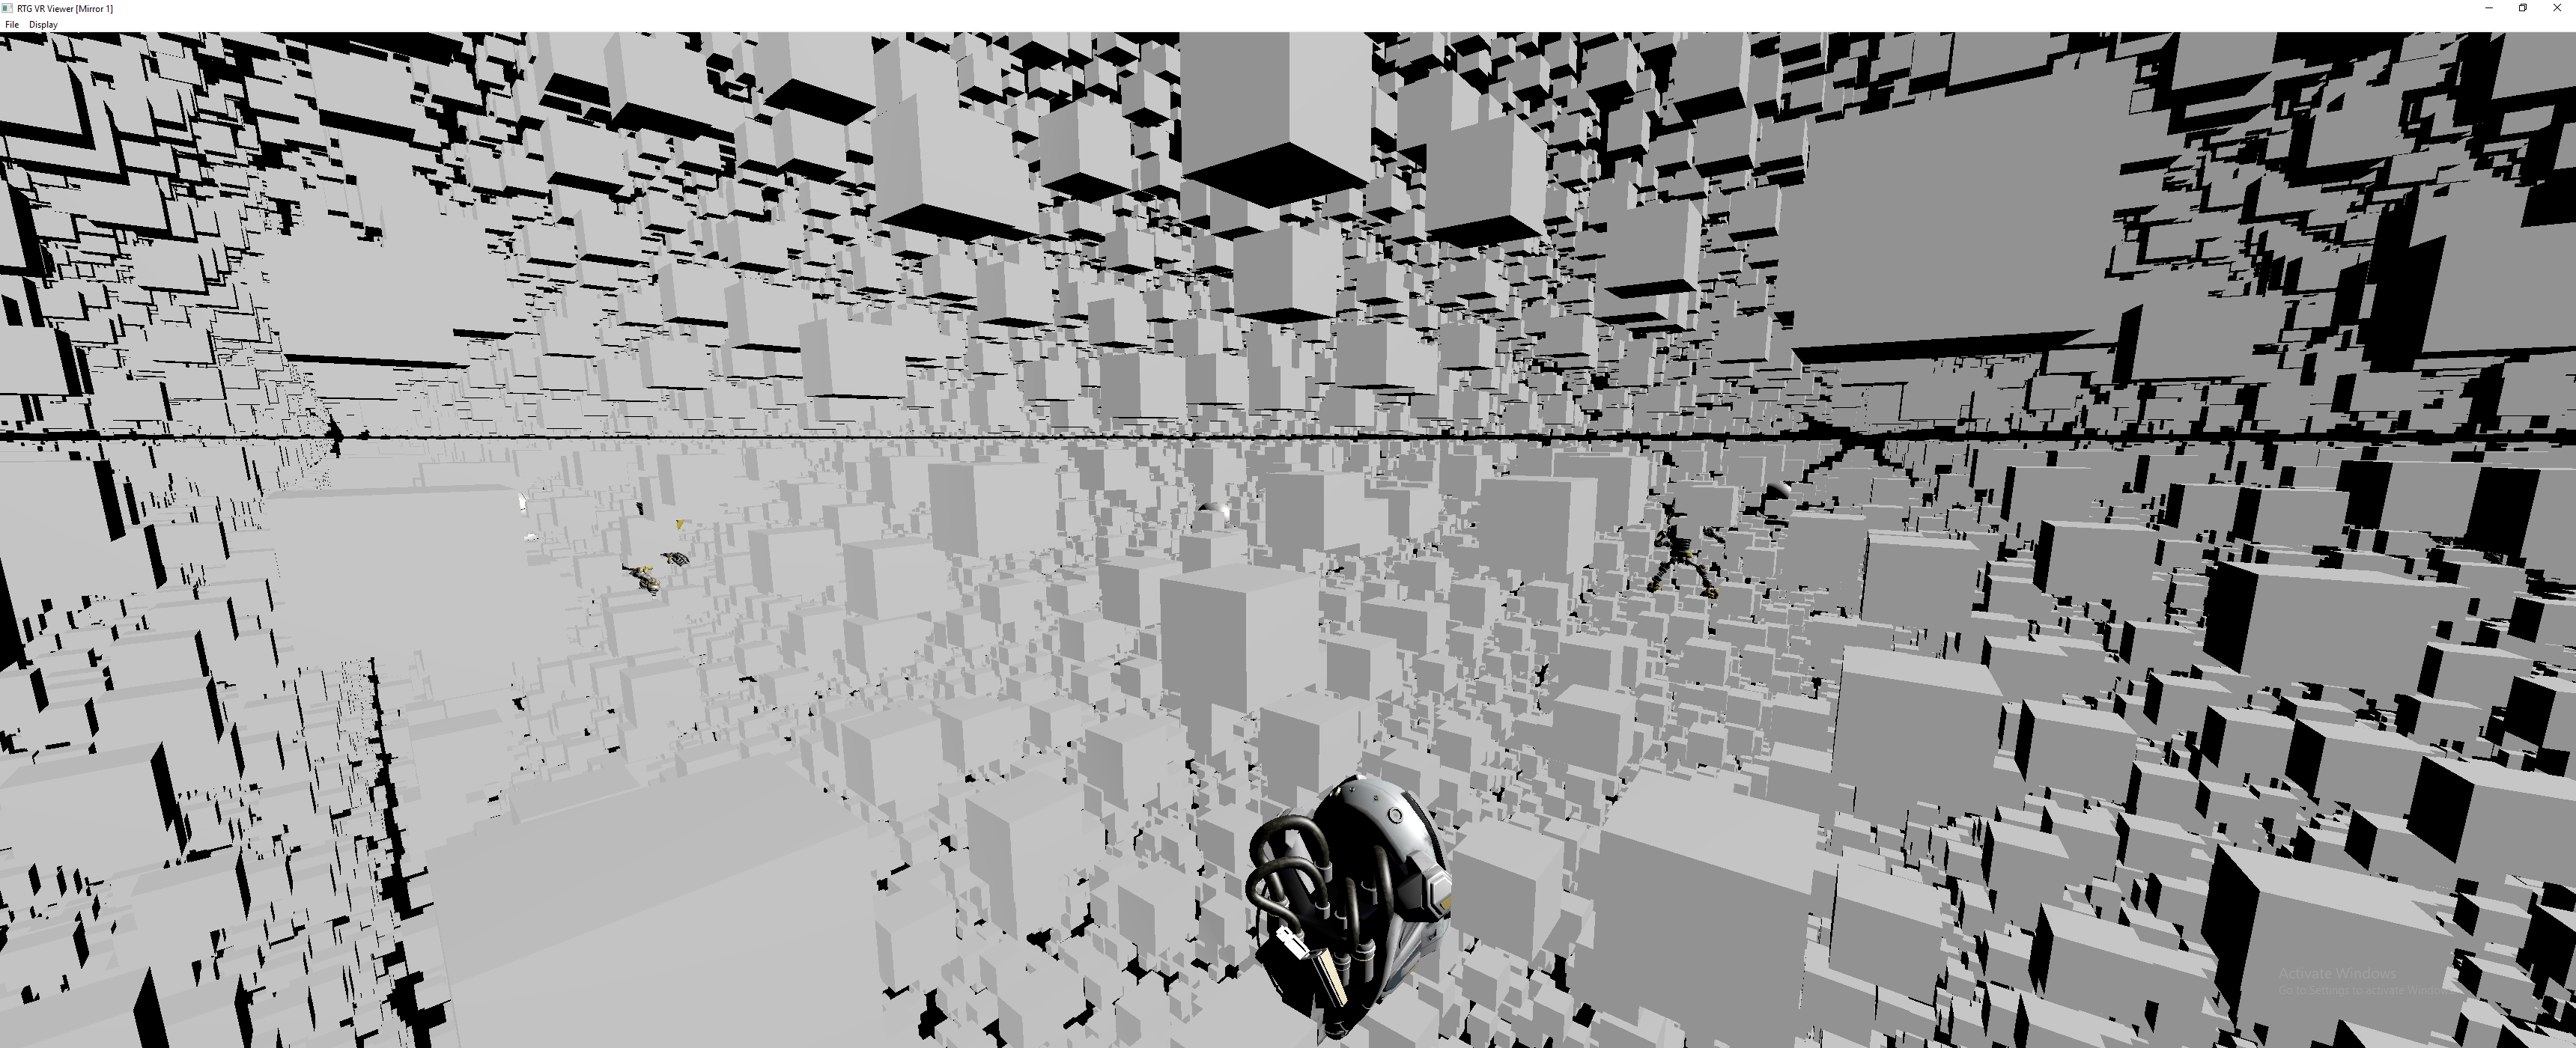
\includegraphics[width=0.8\textwidth]{pictures/scene_chaos}
     }
     \hfill
     \subfloat[The three high polycount assets used in the benchmark scene (LTR: robot "Robi" - 92430 tris, material ball - 46816 tris, glTF2.0 helmet - 15452 tris)\label{fig:highpolys}]{%
       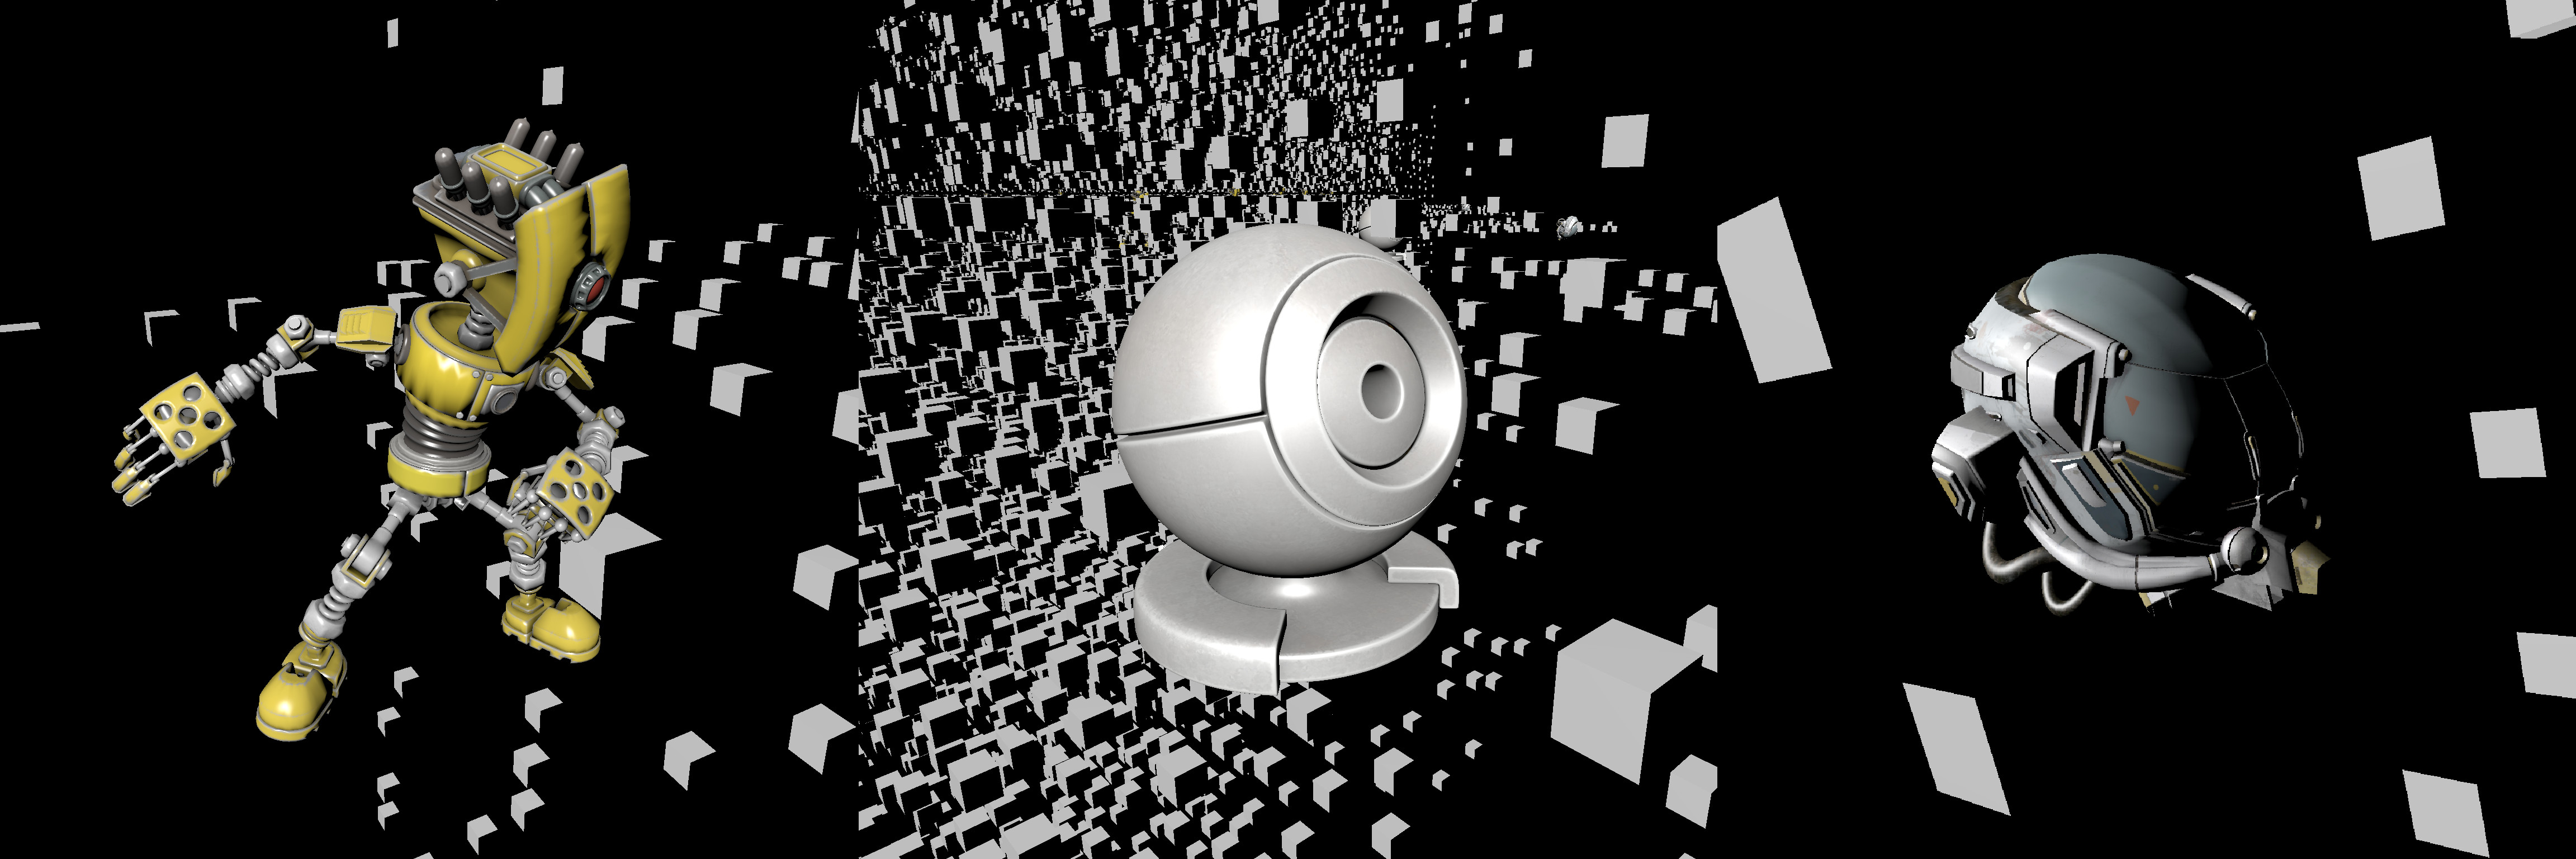
\includegraphics[width=0.8\textwidth]{pictures/highpolys}
     }
     \caption{Benchmark scene details}
     \label{fig:bmark_scene_screencaps}
\end{figure}

\section{Timing code \& metrics} \label{bmark_metrics}
To get an accurate idea of how the computational effort within a frame changes and is split up over its several steps, \codeword{STL::chrono high_resolution_clock} timing calls were used in strategic places. For each frame, the measured metrics are: \begin{itemize}
\item total frame-time (microseconds)
\item CPU-only time (microseconds)
\item Culling-only time (microseconds)
\item GPU-only time (microseconds)
\item number of draw calls submitted
\item number of triangles submitted through draw calls
\end{itemize}
Times are measured by calculating elapsed counts between start and end time points of the respective function call. GPU-only time is measured by artificially placing a \\\codeword{VkQueueWaitIdle(graphicsQueue)} at the end of the \codeword{VKRenderer::RenderFrame} procedure. At first glance this seems counter-productive as it prevents frames from overlapping resource usage, but this is where synthetic repeatability becomes relevant. \\
To guarantee runs with different optimizations enabled can be compared to each other, the render loop is modified to follow aforementioned camera pattern and and save the current frame number with each data point. This obviously flies in the face of desired real-world decoupling of motion from framerate and overlapping execution, but it ensures identical workload per frame for each tested configuration. Additionally, the camera pattern and timings loops are tuned to run exactly twice in exactly 5400 frames each for 10 loops. The resulting 54000 samples of frame data for each configuration are then filtered to exclude the worst outliers and the 10 loops are averaged into one representative set of 5400 data points. The very first frame of the averaged data sets is removed as the very first frame of the first loop after program start includes all initialization commands and major buffer transfers and thus results in an outlier frame time an order of magnitude higher than the remaining 53999 frames of each run. However, in the interest of real-world scaling, a later section will also briefly explore average frametimes for a selection of configurations without these limits in place. \\
Lastly, and this part is crucial, the \codeword{Submit()} calls to SteamVR are disabled for the testing runs as these calls otherwise force vertical refresh synchronization (\autoref{fig:VR_VSync}), completely distorting actual performance numbers. While this means during benchmarking there is no output to the connected HMD, the internal rendering loop still uses all of the HMD's rendering parameters and more importantly renders as many frames as it can without a framerate cap or refresh synchronization, exactly the behavior needed for accurate measurements. 

\begin{figure}[htb]
  \centering
  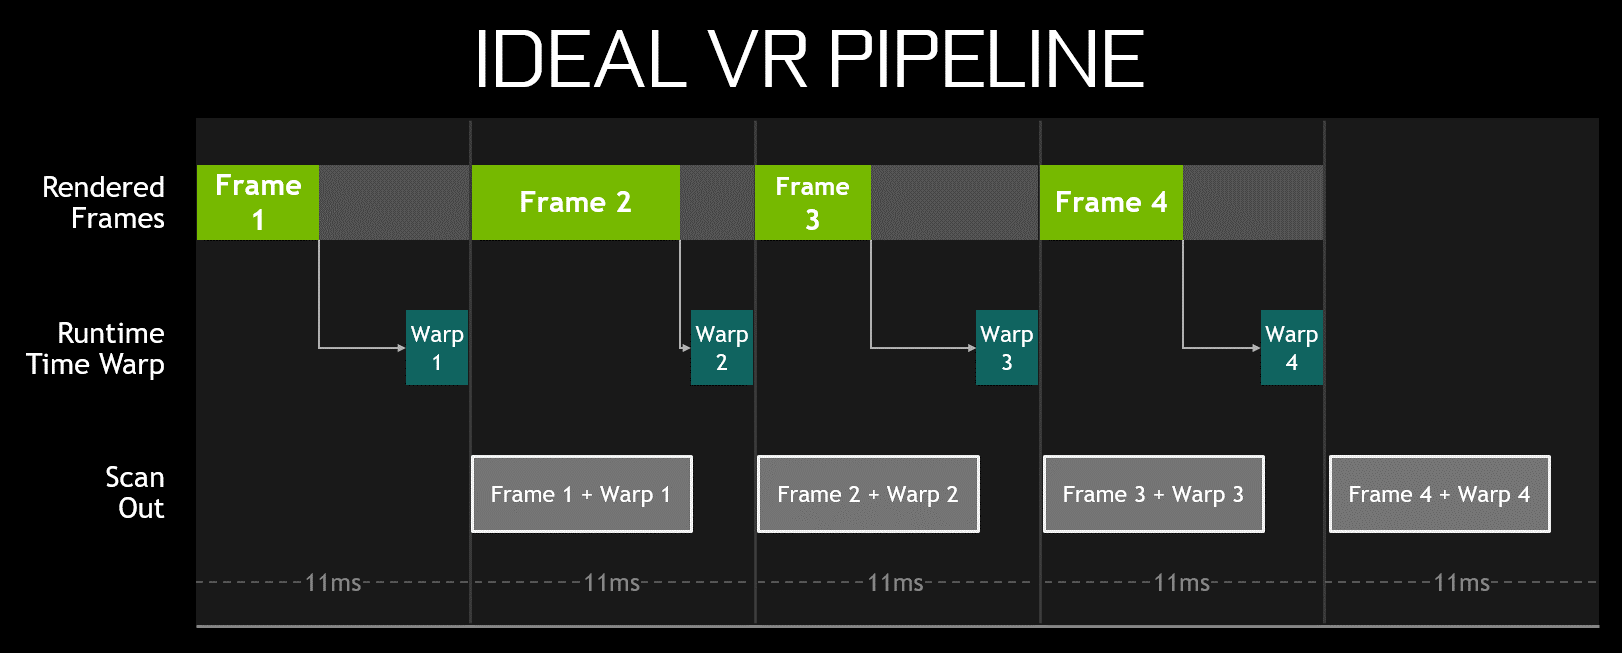
\includegraphics[width=0.9\textwidth]{pictures/Nvidia_FCAT}
  \caption{Virtual Reality Pipeline as imagined by Nvidia (from \cite{Cleveland.2017}, p. 35, S. Cleveland. 2017)} \label{fig:VR_VSync}
\end{figure} 

\section{Compilation parameters}
Naturally productive deployment would go for fastest possible optimization and as such the tested configurations were all compiled with \codeword{-O2} in Release mode using Microsoft Visual Studio 2015 and its v140 MSVC toolset. 
To further eliminate potential slowdown from branching or data tracking, each of the 16 permutations of enabled optimizations is not done simply through \codeword{if} statements or \codeword{switch} cases, but through preprocessor defines. These defines are \codeword{SUPERFRUSTUM_ON}, \codeword{MULTIVIEW_ON}, \codeword{STENCILMASK_ON}, \codeword{MFFR_ON}. Similarly, benchmark timing code is enabled via the \codeword{BENCHMARK_MEASURE}, \codeword{BENCHMARK_CHUNKINFO} and \codeword{BENCHMARK_CAMRAILS} flags. \\
As a sidenote here, all configurations were tested with distance culling (\codeword{DISTANCECULLING_ON}, draw distance 320 units) and frustum culling (\codeword{FRUSTUMCULLING_ON}) enabled as running the massive 11.1 million instance scene without these in place would realistically bring any test machine near a grinding halt. It also seems unrealistic to run any scene with advanced VR optimizations enabled but leave such simple measures disabled. 
Demonstrably, these culling methods are also not posing as dangerous bottlenecks to the tested configurations as the baseline measurement details will show. 

\section{System specifications}
Two test machines were used to test functionality of the optimizations and to perform measurements on. 
The first machine, further titled \textbf{WS-Big}, is specified as:
\begin{itemize}
\item CPU: Intel Core i7 6700 (4c8t Skylake, 4x3.4GHz base, 4.0GHz boost)
\item RAM: 2x16GB DDR4-2400/15
\item GPU: Nvidia GeForce RTX 2080 Founders Edition (2944 Turing cores at 1800MHz core, 8GB GDDR6 at 1750MHz) - driver version 432.00
\item Storage: Samsung SSD 840 Evo 500GB
\item OS: Microsoft Windows 10 Pro x64 1809
\end{itemize} 
The second machine, further titled \textbf{WS-Small}, is specified as:
\begin{itemize}
\item CPU: AMD Ryzen 5 1600 \textit{12nm} (6c12t Zen+, 6x3.2GHz base, 3.7GHz boost)
\item RAM: 2x8GB DDR4-3066/14
\item GPU: Hewlett-Packard Radeon RX 580 (2304 Polaris cores at 1200MHz, 4GB GDDR5 at 1750MHz) - driver version 20.1.3
\item Storage: ADATA SSD SX6000 Pro 500GB
\item OS: Microsoft Windows 10 Pro x64 1909
\end{itemize} 
Furthermore, the following virtual reality headsets were available with the respective internal per-eye resolution setting and in the respective capacity:
\begin{itemize}
\item Valve Index (2016x2240 pixels)) - \textbf{WS-Big} performance measurements, functionality verification
\item HTC Vive (1512x1680 pixels) - \textbf{WS-Big} functionality verification
\item HTC Vive Pro (2016x2240 pixels) - \textbf{WS-Big} functionality verification
\item Oculus Rift CV1 (1344x1600 pixels) - \textbf{WS-Big} \& \textbf{WS-Small} functionality testing
\item Samsung Odyssey (1449x1797 pixels) - \textbf{WS-Small} functionality testing
\end{itemize} 
To ensure repeatability and level the field as much as possible, the CPU of each system is locked to a fixed clock multiplier and thus operating frequency. For the i7 6700 and its lack of unlocked multiplier this is achieved by setting minimum and maximum processor state in Windows to 100 and 99\% respectively, which effectively disables singlecore turbo boost and speedshift and fixates the frequency at the allcore boost multiplier of 37x for 3.7GHz allcore. For the Ryzen 5 1600 a more reliable method is available, that being manually overriding the CPU multiplier within the mainboard UEFI, in this case to a fixed value of 38x for 3.8GHz across all 12 processor threads. \\
Keeping GPU clock speeds at the same level for all test runs is harder to achieve as all modern graphics cards employ some version of dynamic boosting algorithms based on temperature, power target, voltage target and usage. The Radeon RX 580 is set to target a maximum of 1200MHz boost frequency via a VBIOS modification that disables higher automatic boost, and during core load it maintains this target stable unless the power target of 100 Watts is exceeded. 
For Nvidia graphics cards later than 2014's Maxwell 2 architecture, such a firmware mod is unfortunately not possible. There is, however, one way of reaching a mostly stable core frequency. To achieve this, the card needs to be pre-heated using any application generating GPU load. To prime \textbf{WS-Big}'s RTX 2080, SteamVR Home is idled for 30 minutes before any test runs are performed, resulting in an equilibrium of \ang{70}C at 1905MHz core frequency. This temperature and frequency is maintained for the entirety of each test run as the 210 Watts power target of the card is never exceeded. 